\documentclass[11pt,a4paper]{article}
\usepackage[UTF8]{ctex}
\usepackage{amsmath,amssymb}
\usepackage{graphicx}
\usepackage{hyperref}

\title{dsh-leaf 示例论文\\\large 从实验到投稿的一体化写作工作区}
\author{dsh-leaf}
\date{\today}

\begin{document}
\maketitle

\begin{abstract}
This is the minimal example project for dsh-leaf, intended to validate workspace detection, section organization, figure preview, the compilation pipeline, and PDF preview. The data shown in the figures are illustrative values and do not represent real experimental results.
\end{abstract}

\section{引言}
\label{sec:intro}

投稿准备通常横跨实验代码、数据、图表与论文源码多个目录。dsh-leaf 将整个目录视为一个
LaTeX 项目：普通对话负责实验与绘图，写作视图负责源码、编译与 PDF 审阅。

本文的主要观察是：把编译入口固定为主文档，并让章节文件共享同一个写作视图，可以显著减少
在多个工具之间搬运上下文的时间。示意结果见图~\ref{fig:workflow}。

\begin{figure}[htbp]
  \centering
  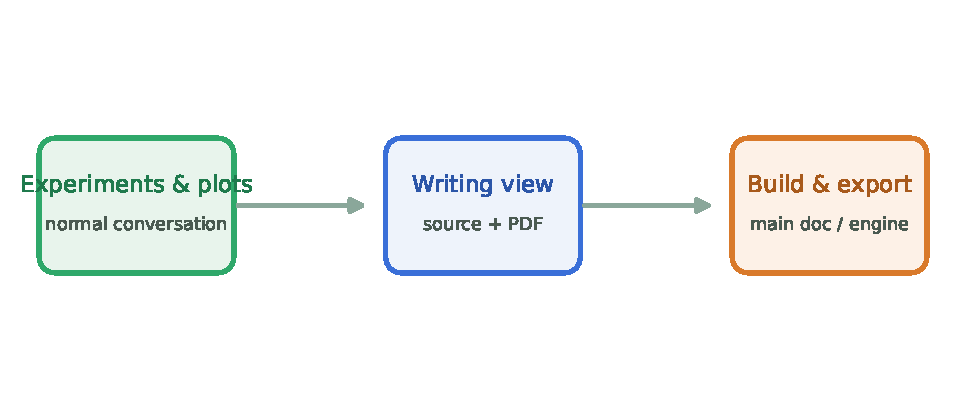
\includegraphics[width=0.72\linewidth]{figures/workflow.pdf}
  \caption{dsh-leaf 的工作流程示意：资料整理、绘图、写作、编译与导出共享同一个工作区。}
  \label{fig:workflow}
\end{figure}

相关工作可参考~\cite{lamport1994latex}。

\section{方法}
\label{sec:method}

设工作区中的主文档为 $M$，章节集合为 $S=\{s_1,\dots,s_n\}$。编译过程总是从 $M$ 出发，
按引用关系展开 $S$ 与图片资源：
\begin{equation}
  \mathrm{Build}(M) = \mathrm{PDF}\bigl(M \cup \mathrm{deps}(M)\bigr).
  \label{eq:build}
\end{equation}

式~\eqref{eq:build} 说明，章节标签的点击不会改变编译入口；它只是切换到对应的源码位置。
快速模式将外部图片替换为占位框，但保留文字与公式排版，导出时始终回到完整编译结果。


\bibliographystyle{plain}
\bibliography{references}

\end{document}
